%%%%%%%%%%%%%%%%%%%%%%%%%%%%%%%%%%%%%%%%%
% Beamer Presentation
% LaTeX Template
% Version 1.0 (10/11/12)
%
% This template has been downloaded from:
% http://www.LaTeXTemplates.com
%
% License:
% CC BY-NC-SA 3.0 (http://creativecommons.org/licenses/by-nc-sa/3.0/)
%
%%%%%%%%%%%%%%%%%%%%%%%%%%%%%%%%%%%%%%%%%

%----------------------------------------------------------------------------------------
%	PACKAGES AND THEMES
%----------------------------------------------------------------------------------------

\documentclass{beamer}

\mode<presentation> {

% The Beamer class comes with a number of default slide themes
% which change the colors and layouts of slides. Below this is a list
% of all the themes, uncomment each in turn to see what they look like.

%\usetheme{default}
%\usetheme{AnnArbor}
%\usetheme{Antibes}
%\usetheme{Bergen}
%\usetheme{Berkeley}
%\usetheme{Berlin}
%\usetheme{Boadilla}
%\usetheme{CambridgeUS}
%\usetheme{Copenhagen}
%\usetheme{Darmstadt}
%\usetheme{Dresden}
\usetheme{Frankfurt}
%\usetheme{Goettingen}
%\usetheme{Hannover}
%\usetheme{Ilmenau}
%\usetheme{JuanLesPins}
%\usetheme{Luebeck}
%\usetheme{Madrid}
%\usetheme{Malmoe}
%\usetheme{Marburg}
%\usetheme{Montpellier}
%\usetheme{PaloAlto}
%\usetheme{Pittsburgh}
%\usetheme{Rochester}
%\usetheme{Singapore}
%\usetheme{Szeged}
%\usetheme{Warsaw}

% As well as themes, the Beamer class has a number of color themes
% for any slide theme. Uncomment each of these in turn to see how it
% changes the colors of your current slide theme.

%\usecolortheme{albatross}
%\usecolortheme{beaver}
%\usecolortheme{beetle}
%\usecolortheme{crane}
%\usecolortheme{dolphin}
%\usecolortheme{dove}
%\usecolortheme{fly}
%\usecolortheme{lily}
%\usecolortheme{orchid}
%\usecolortheme{rose}
%\usecolortheme{seagull}
%\usecolortheme{seahorse}
%\usecolortheme{whale}
%\usecolortheme{wolverine}

%\setbeamertemplate{footline} % To remove the footer line in all slides uncomment this line
%\setbeamertemplate{footline}[page number] % To replace the footer line in all slides with a simple slide count uncomment this line

%\setbeamertemplate{navigation symbols}{} % To remove the navigation symbols from the bottom of all slides uncomment this line
}

\usepackage{graphicx} % Allows including images
\usepackage{booktabs} % Allows the use of \toprule, \midrule and \bottomrule in tables
\usepackage{color}
\usepackage[ruled, vlined, linesnumbered]{algorithm2e}
\usepackage{subfig}
\usepackage{pgf}
\usepackage{multirow}
%\usepackage[a4paper,top=10.0mm,bottom=15.0mm]{geometry}


%\newtheorem{theorem}{Theorem}
\newtheorem{protocol}{Protocol}
%\newtheorem{lemma}{Lemma}
\newtheorem{claim}{Claim}
\newtheorem{property}{Property}



\newcommand{\bbZ}{\mathbb{Z}}
\newcommand{\calC}{\mathcal{C}}
\newcommand{\calI}{\mathcal{I}}
\newcommand{\calM}{\mathcal{M}}
\newcommand{\calK}{\mathcal{K}}
\newcommand{\opt}{\text{OPT}}
\newcommand{\knowopt}{{\sc KnowOpt}}
\newcommand{\alg}{\text{ALG}}
\newcommand{\E}{\mathbf{E}}
\newcommand{\emRed}[1][]{\textcolor{blue} #1}
\newcommand{\bbR}{\mathbb{R}}
\newcommand{\eps}{\epsilon}
\newcommand{\greedy}{{\sc Greedy}~}
\newcommand{\greedyLazy}{{\sc GreedyLazy}~}
\newcommand{\stocGreedy}{{\sc StocGreedy}~}
%\newcommand{\baseline}{{\sc BaselineStream}~}
\newcommand{\randomSampling}{{\sc RandomSampling}~}
\newcommand{\sieveStream}{{\sc SieveStream}~}
\newcommand{\sieveStreamOPT}{{\sc SieveStreamOPT}~}
\newcommand{\randomStream}{{\sc RandomStream}~}
\newcommand{\circuitStream}{{\sc CircuitStream}~}
\newcommand{\offline}{{\sc Offline}~}

\DeclareMathOperator*{\argmin}{arg\,min}
\DeclareMathOperator*{\argmax}{arg\,max}
\newcommand{\chensays}[2][]{\textcolor{red} {\textsc{Chen #1:} \emph{#2}}}
%----------------------------------------------------------------------------------------
%	TITLE PAGE
%----------------------------------------------------------------------------------------

\title[Submodular Maximization]{Submodular Maximization\\\small{advances in distributed/streaming computing}} % The short title appears at the bottom of every slide, the full title is only on the title page

\author{Jiecao Chen} % Your name
\institute[IUB] % Your institution as it will appear on the bottom of every slide, may be shorthand to save space
{
Indiana University Bloomington \\ % Your institution for the title page
\medskip
\textit{jiecchen@indiana} % Your email address
}
\date{\today} % Date, can be changed to a custom date

\begin{document}

\begin{frame}
\titlepage % Print the title page as the first slide
\end{frame}

\begin{frame}
\frametitle{Overview} % Table of contents slide, comment this block out to remove it
\tableofcontents % Throughout your presentation, if you choose to use \section{} and \subsection{} commands, these will automatically be printed on this slide as an overview of your presentation
\end{frame}

%----------------------------------------------------------------------------------------
%	PRESENTATION SLIDES
%----------------------------------------------------------------------------------------

%------------------------------------------------
\section{Introduction to Submodularity} % Sections can be created in order to organize your presentation into discrete blocks, all sections and subsections are automatically printed in the table of contents as an overview of the talk
%------------------------------------------------

\subsection{Definitions \& Properties} % A subsection can be created just before a set of slides with a common theme to further break down your presentation into chunks

\begin{frame}
\frametitle{Definitions of Submodularity}
\begin{definition}[submodular concave]
  \label{def:sub-concave}
  A function $f:~2^V \rightarrow \bbR$ is \emRed{submodular} if for any $A, B \subseteq V$, we have that:
  \begin{equation}
    \label{eq:sub-concave}
    f(A) + f(B) \geq f(A \cup B) + f(A \cap B).
  \end{equation}
\end{definition}

\pause
An alternate equivalent definition is more interpretable in many situations.

\begin{definition}[diminishing returns]
  \label{def:sub-diminishing}
  A function $f: 2^V \rightarrow \bbR$ is \emRed{submodular} if for any $A \subseteq B \subset V$, and $v \in V\backslash B$, we have that:
  \begin{equation}
    \label{eq:sub-diminishing}
    f(A + v) - f(A) \geq f(B + v) - f(B).
  \end{equation}
\end{definition}

\end{frame}

%------------------------------------------------

% \begin{frame}
% \frametitle{Modular Functions}
% \begin{definition}[Modularity]
%   \label{def:modular}
%   A function $f: 2^V \rightarrow \bbR$ is \emRed{modular} if for any $A \subseteq B \subset V$, and $v \in V\backslash B$, we have that:
%   \begin{equation}
%     \label{eq:modular}
%     f(A + v) - f(A) = f(B + v) - f(B).
%   \end{equation}
% \end{definition}
% Notably, a modular function $f$ can always be written as
% $$f(S) = f(\emptyset) + \sum_{v\in S} \left( f(\{v\}) - f(\emptyset) \right)$$
% for any $S \subseteq V$. If we further assume $f(\emptyset) = 0$ (in this case, we call $f$ \emRed{normalized} or \emRed{proper}), we have a simplified expression,

% $$f(S) = \sum_{v\in S} f(\{v\}).$$
% \end{frame}

% \begin{frame}
% \frametitle{Monotonitcity}
% \begin{definition}[Monotonitcity]
%   A set function $f: 2^V \rightarrow  \bbR$ is said to be non-decreasing if for any $A\subseteq B \subseteq V$, $f(A) \leq f(B)$. Non-increasing set functions are defined in the similar way.
% \end{definition}
% When we say a submodular function is monotone, we mean it is non-decreasing.
% \end{frame}


%\subsection{Properties}
\begin{frame}
\frametitle{Properties}

Submodularity is closed under addition.
\begin{property}
  \label{prop:addition}
  Let $f_1, f_2: 2^V \rightarrow \bbR$ be two submodular functions. Then 
  $$f: 2^V\rightarrow \bbR~~\text{with}~~ f(A) = \alpha f_1(A) + \beta f_2(A)$$ 
is submodular for any fixed $\alpha, \beta \in \bbR^+$.
\end{property}
\pause
Submodularity is preserved under restriction.
\begin{property}
  \label{prop:restriction}
  Let $f: 2^V \rightarrow \bbR$ be a submodular function. Let $S\subseteq V$ be a fixed set. Then
$$f':2^V \rightarrow \bbR~~\text{with}~~f'(A) = f(A\cap S)$$
is submodular.
\end{property}
\end{frame}


\begin{frame}
\frametitle{Properties cont.}
The following property can be useful if we want to show that the negative of the objective function of k-median problem is submodular.
\begin{property}
  \label{prop:max}
Let $V$ be the ground set we consider, each element in $V$ is a real number.  Then 
$$f:2^V \rightarrow \bbR~~\text{with}~~ f(A) = \max_{c\in A}c$$ 
is submodular.
\end{property}
\end{frame}



\subsection{Constraints}
\begin{frame}
\frametitle{Constraints}
\begin{block}{Submodular Maximization Problem}
A submodular maximization problem usually has the following form:

\begin{equation}
  \label{eq:optimization}
  \argmax_{I\in\calI} f(I),
\end{equation}
\end{block}
where $f$ is a submodular function and $\calI \subseteq 2^V$ is the collection of all feasible solutions. We call $\calI$ the \emRed{constraint} of the optimization problem.
  \begin{block}{Example}
    \emRed{Cardinality constraint}: $\calI = \{A \subseteq V ~|~ |A| \leq k\}$
  \end{block}
  \pause

\end{frame}


\begin{frame}
\frametitle{Constraints}

\begin{block}{$\calI$ is important!}
The structure of $\calI$ plays a crucial role in submodular optimization:
\begin{itemize}
\item Different constraints have different hardness results.
\item Normally the difficulty increases when the constraint becomes more general.
\end{itemize}
\end{block}
\pause
\begin{block}{Popular constraints}
Some popular constraints:
\begin{itemize}
\item Cardinality constraint
\item Knapsack constraint
\item Matroid constraint
\item Matching
\item $p$-System
\item ...
\end{itemize}
\end{block}
\end{frame}



\begin{frame}
\frametitle{Constraints cont.}
First we define hereditary set systems.
\begin{definition}[Hereditary]
  \label{def:hereditary}
  A constraint $\calI \subseteq 2^V$ is said to be \emRed{hereditary} if 
$$I\in\calI \implies J\in\calI ~\text{for any}~J\subseteq I.$$
A hereditary constraint is sometimes called an \emRed{independent system} and each $I\in\calI$ is called an \emRed{independent set}. 
\end{definition}
\textbf{All constraints we will discuss are hereditary.}
\end{frame}

\begin{frame}
  \frametitle{Constraints cont.}
\begin{block}{Cardinality}
    \emRed{Cardinality constraint}: $\calI = \{A \subseteq V ~|~ |A| \leq k\}$
  \end{block}
  \pause
  \begin{block}{Knapsack}
   \emRed{Knapsack Constraint}: each $i \in V$ is assigned a weight $w_i \geq 0$,  $\calI = \{S \subseteq V ~|~ \sum_{i\in S} w_i \leq W \}$.
  \end{block}

  \pause

  \begin{block}{Matching}
     \emRed{Matching}: given a graph $G = (V, E)$, a \emph{Matching} is a set $S\subseteq E$ such that no edges in $S$ share common vertex.
  \end{block}
  \pause
  \begin{block}{Matroid}
    \emRed{Matroid} is the generalization of the independence concept in linear algebra;
    omit details here ...
  \end{block}


\end{frame}




\begin{frame}
  \frametitle{$p$-System}
\emRed{$p$-system} is very general, it includes many other constraints as special cases.

\begin{block}{Definition of $p$-System}
Let $(V, \calI)$ be a set system and $\calI$ hereditary.  Let $\mathcal{B}(A)$ be the collection of all bases of $A$.

$$\calI = \{ A \subseteq V ~|~ \frac{\max_{S\in\mathcal{B}(A)}|S|}{\min_{S\in\mathcal{B}(A)}|S|} \leq p \}.$$
\end{block}
\pause
\textbf{Note:} a \emRed{base} of $A$ is the maximal independent set included in $A$. 
\pause
\begin{block}{examples of $p$-system}
  \begin{itemize}
    \item matroid is $1$-system
    \item matching is $2$-system
    \item intersection of $p$ matroids is $p$-system
    \item ...
  \end{itemize}
\end{block}
\end{frame}


\begin{frame}
  \frametitle{Hierarchy of constraints}
  \begin{figure}[!ht]
    \centering
    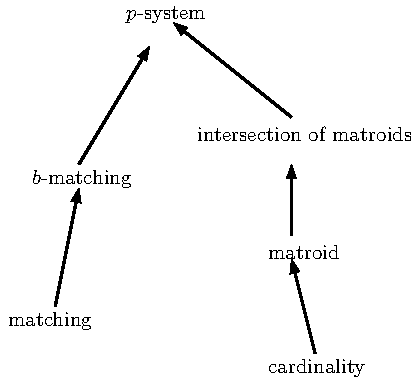
\includegraphics[width=0.7\textwidth]{figures/hh}
  \end{figure}
\end{frame}


\begin{frame}
  \frametitle{Hierarchy of constraints (extended)}
  \begin{figure}[!ht]
    \centering
    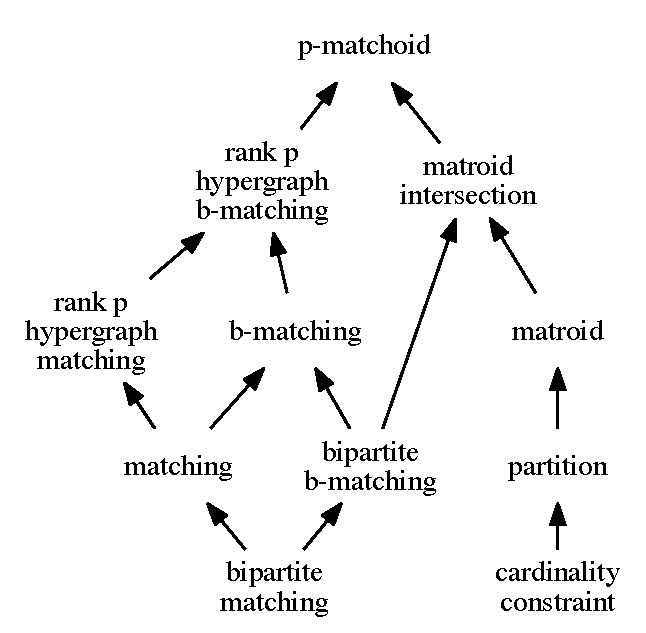
\includegraphics[width=0.7\textwidth]{figures/hierarchy}
  \end{figure}
\end{frame}


%------------------------------------------------



\subsection{Algorithms}

\begin{frame}
  \frametitle{Notations}
  \begin{block}{Some notations}
    \begin{itemize}
      \item $\Delta_f(e|S) = f(S + e) - f(S)$ (or simply $\Delta(e|S)$ when $f$ is clear from context), call it \emRed{marginal gain}.
      \item \emRed{$\alpha$-approximation}: the returned solution $S$ always satisfies  $f(S) \geq \alpha \cdot \argmax_{I\in\calI}f(I)$
      \item When the algorithm is randomized, we normally say it guarantees \emRed{$\alpha$-approximation in expectation} if $$\E[f(S)] \geq \alpha\cdot \argmax_{I\in\calI}f(I).$$ 
    \end{itemize}
  \end{block}
\end{frame}


\begin{frame}
  \frametitle{The standard greedy algorithm}
  \begin{algorithm}[H]
    \DontPrintSemicolon % Some LaTeX compilers require you to use \dontprintsemicolon instead
    \KwIn{$V$ the ground set, $f$ the submodular function, $\calI$ the constraint}
    \KwOut{a set $S \subseteq V$}
    $S \gets \emptyset$\;
    \While{$\exists ~e\in V\backslash S$ s.t. $S\cup\{e\}\in \calI$} {
      $e \gets \argmax_{e\in V\backslash S, ~S\cup\{e\}\in \calI} \Delta_f(e|S)$\;\label{line:emax}
      $S \gets S\cup \{e\}$\;
    }
    \Return{$S$}\;
    \caption{{\sc Greedy} algorithm for submodular maximization}
    \label{algo:greedy}
\end{algorithm}

\end{frame}

\begin{frame}
  \frametitle{Theorems of Algorithm \ref{algo:greedy}}
\begin{theorem}[\cite{NWF78}, for cardinality constraint]
  \label{thm:1978}
  For a non-negative \emRed{monotone submodular} function $f: 2^V \rightarrow \bbR$, let $\calI$ be the \emRed{cardinality constraint}, Algorithm \ref{algo:greedy} returns a $(1 - 1/e)$-approximation to $\argmax_{I\in \calI} f(S)$.
\end{theorem}
\pause
\begin{theorem}[\cite{NWF78,CCP+11}, for $p$-system]
  \label{thm:1978-p}
  For a non-negative \emRed{monotone submodular} function $f$, given a $p$-system $(V, \calI)$, Algorithm \ref{algo:greedy} returns a $\frac{1}{p + 1}$-approximation.
\end{theorem}
% \pause
% \begin{theorem}[\cite{J76}, modular maximization s.t. $p$-system]
%   \label{thm:1976-p}
%   For a non-negative \emRed{monotone modular} function $f$, given a $p$-system $(V, \calI)$, Algorithm \ref{algo:greedy} returns a $\frac{1}{p}$-approximation.
% \end{theorem}
\end{frame}


\begin{frame}
 \frametitle{Speedup - {\sc GreedyLazy}}
 \begin{block}{GreedyLazy}
   \begin{itemize}
   \item<1,2,3,4>  Minoux \cite{M78} proposed {\sc Lazy-greedy} as a fast implementation for Algorithm \ref{algo:greedy}.
   \item<2,3,4> {\sc GreedyLazy} keeps an upper bound $\rho(e)$ on the marginal gain sorted in a heap.
    \item<3,4> In each step, only update the top element in the heap and push it back, if this element remains in the top, include it into solution.
    \item<4> Again gives $(1 - e^{-1})$-approximation.
   \end{itemize}
 \end{block}
\end{frame}

\begin{frame}
\frametitle{Speedup - {\sc StocGreedy}\cite{MBK+15}}
 \begin{block}{StocGreedy}
   \begin{itemize}
   \item<1,2,3> In each round, instead of considering all $V\backslash S$  to get
     $$e \gets \argmax_{e\in V\backslash S, ~S\cup\{e\}\in \calI} \Delta_f(e|S),$$
    \item<2,3>   consider only $\frac{|V|}{k}\log\frac{1}{\epsilon}$ random samples from $V \backslash S$.
    \item<3> $(1 - e^{-1}-\epsilon)$-approximation in expectation.
   \end{itemize}
\end{block}
 \end{frame}



 \begin{frame}
   \frametitle{Comparison}
\begin{figure}[h!t]
     \centering
     \subfloat[][Efficiency]{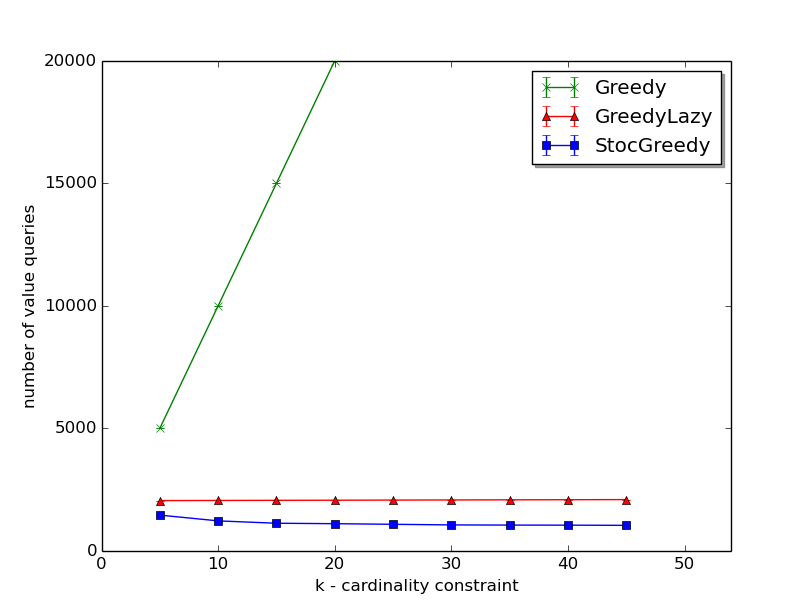
\includegraphics[width=0.5\textwidth]{figures/value-queries}\label{fig:greedy-efficiency}}
     ~~
     \subfloat[][Quality]{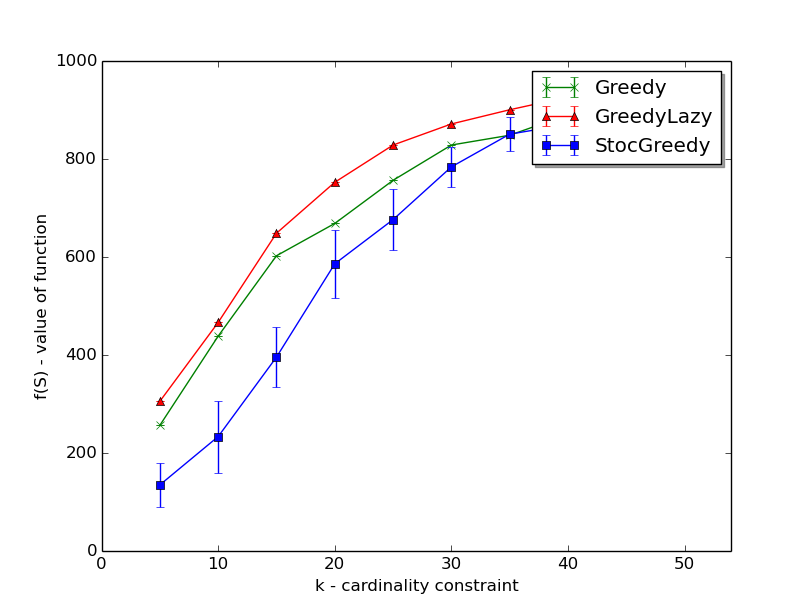
\includegraphics[width=0.5\textwidth]{figures/func-values}\label{fig:quality-greedy}}    
     \caption{Experiment on {\sc Synthetic} dataset}
     \label{fig:sythetic-offline}
   \end{figure}
 \end{frame}




\begin{frame}
  \frametitle{Summary of state of the arts}
  \begin{table}[t]
\centering
\begin{tabular}{|l|l|l|}
\hline
constraint & monotone  &  non-negative \\
\hline
cardinality & $1 - 1/e$  \cite{NWF78} & $1/e + .004$ \cite{BFN+14}\\
\hline
matroid & $1 - 1/e$ \cite{CCP+11}, R & $\frac{1 - \eps}{e}$ \cite{FNS11}, R \\
\hline
matching & $\frac{1}{2 + \eps}$ \cite{FNS+11} & $\frac{1}{4 + \eps}$ \cite{FNS+11}\\
\hline
intersection of $p$ matroids & $\frac{1}{p + \eps}$ \cite{LSV10} & $\frac{p - 1}{p^2 + \eps}$ \cite{LSV10}\\
\hline
$p$-matchoid & $\frac{1}{p + 1}$ \cite{CCP+11,NWF78} & $\frac{(1-\eps)(2-o(1))}{e\cdot p}$ \cite{FNS+11,VCZ11}, R\\
\hline
\end{tabular}
\caption{Best known approximation bounds for submodular maximization in RAM model. Bounds for randomized algorithms that hold in expectation are marked (R).}
\label{table:centralized}
\end{table}
\end{frame}

% \begin{frame}
% \frametitle{Multiple Columns}
% \begin{columns}[c] % The "c" option specifies centered vertical alignment while the "t" option is used for top vertical alignment

% \column{.45\textwidth} % Left column and width
% \textbf{Heading}
% \begin{enumerate}
% \item Statement
% \item Explanation
% \item Example
% \end{enumerate}

% \column{.5\textwidth} % Right column and width
% Lorem ipsum dolor sit amet, consectetur adipiscing elit. Integer lectus nisl, ultricies in feugiat rutrum, porttitor sit amet augue. Aliquam ut tortor mauris. Sed volutpat ante purus, quis accumsan dolor.

% \end{columns}
% \end{frame}

%------------------------------------------------
\section{Applications}
%------------------------------------------------
\subsection{Overview}
\begin{frame}
\frametitle{Overview of Applications}
%\subsection{List of Possible Applications}
\begin{itemize}
\item \textbf{Combinatorial Problems}: set cover, max $k$ coverage, vertex cover, edge cover, graph cut problems etc.
\item \textbf{Networks}: social networks, viral marketing, diffusion networks etc.
\item \textbf{Graphical Models}: image segmentation, tree distributions, factors etc.
\item \textbf{NLP}: document summarization, web search, information retrieval
\item \textbf{Machine Learning}: active/semi-supervised learning etc.
\item \textbf{Economics}: markets, economies of scale
\end{itemize}

\end{frame}

%------------------------------------------------
\subsection{Examples of Applications}
\begin{frame}
\frametitle{Set Cover Problem}
\begin{itemize}
\item Let $E$ be a fixed set with finite size.
\item $V = \{C_1, C_2, \ldots, C_n\}$ where each $C_i \subseteq E$.
\item  We define a function $f:2^V \rightarrow \bbR$ such that $f(S) = |\cup_{C\in S} C|$.
\item Goal: pick $S \subseteq V$ with $|S| \leq k$ that maximizes $f(S)$
\item $f(S)$ is monotone submodular and this is a submodular maximization problem s.t. cardinality constraint!
\end{itemize}

\end{frame}


\begin{frame}
\frametitle{Kernel Machines}
The data set $V = \{x_1, x_2, \ldots, x_n\}$ is represented in a transformed space via a kernel matrix

\[ K_V = \left( \begin{array}{ccc}
\calK(x_1, x_2) & \ldots & \calK(x_1, x_n) \\
\vdots & \ddots & \vdots \\
\calK(x_n,x_1) & \ldots & \calK(x_n, x_n) \end{array} \right),\] 
where $\calK: V\times V \rightarrow \bbR$ is the kernel function that is symmetric and positive definite. 
\end{frame}

\begin{frame}
  \frametitle{Kernel Machines cont.}
  \begin{itemize}
  \item   $K_V$ is large for large $|V|$, need to select a subset from $V$.
  \item   How to measure the quality of selected subset?
  \item A popular way is to use \emph{Informative Vector Machine} (IVM) introduced by Laurence et al.\ \cite{LSH03}:
    $$f(S) = \frac{1}{2} \log\det\left( \mathbf{I} + \sigma^{-2} K_S \right)$$
   \item $f(S)$ is submodular!
   \item Goal: $$\argmax_{S\subseteq V : |S| \leq k} f(S).$$
  \end{itemize}

\end{frame}








%------------------------------------------------


% \begin{frame}[fragile] % Need to use the fragile option when verbatim is used in the slide
% \frametitle{Verbatim}
% \begin{example}[Theorem Slide Code]
% \begin{verbatim}
% \begin{frame}
% \frametitle{Theorem}
% \begin{theorem}[Mass--energy equivalence]
% $E = mc^2$
% \end{theorem}
% \end{frame}
% \end{verbatim}
% \end{example}
% \end{frame}

%------------------------------------------------

% \begin{frame}
% \frametitle{Figure}
% Uncomment the code on this slide to include your own image from the same directory as the template .TeX file.
% %\begin{figure}
% %\includegraphics[width=0.8\linewidth]{test}
% %\end{figure}
% \end{frame}

%------------------------------------------------

% \begin{frame}[fragile] % Need to use the fragile option when verbatim is used in the slide
% \frametitle{Citation}
% An example of the \verb|\cite| command to cite within the presentation:\\~

% This statement requires citation \cite{p1}.
% \end{frame}

%------------------------------------------------
%------------------------------------------------
\section{Streaming Submodular Maximization}
%------------------------------------------------
\subsection{Streaming Model} 
\begin{frame}{The model}

  The ground set $V$ is an ordered sequence of items $e_1, e_2, \ldots, e_n$. We process the items one by one and the maximum space being used should be sublinear (i.e. $o(n)$).
\begin{figure}[p]
    \centering
    \includegraphics[width=0.8\textwidth]{figures/streaming-model.pdf}
    \caption{Streaming model}
    \label{fig:streaming-model}
\end{figure}

\end{frame}


\subsection{Algorithms}

\begin{frame}
\frametitle{\sieveStream assume $\opt$ is known}
\begin{algorithm}[H]
\DontPrintSemicolon % Some LaTeX compilers require you to use \dontprintsemicolon instead
\KwIn{$V$ as data stream, $f$ a monotone submodular function, $k$ the size constraint, $\opt$ the optimal value of $f(S)$ under the constraint}
\KwOut{a set $S \subseteq V$}
$S \gets \emptyset$\;
\For{each $e$ in the data stream} {
  \If{$\Delta(e|S) \geq \frac{\opt/2 - f(S)}{k - |S|}$ and $|S|<k$}{
      $S \gets S \cup \{e\}$\;    
    }
}
\Return{$S$}\;
\caption{\sieveStreamOPT for submodular maximization}
\label{algo:sieveStreamOPT}
\end{algorithm}
\end{frame}

\begin{frame}
  \frametitle{\sieveStream assume $\opt$ is unknown}
  \begin{block}{Problems with \sieveStreamOPT}
    \large{$\opt$ is unknown!}
  \end{block}
  \pause
  So what we do?    
  \pause
  \begin{block}{Solution}
    \begin{itemize}
    \item $m = \max_{e\in V}f(\{e\})$, for simplicity, assume $f(\emptyset) = \emptyset$
    \item note that $m \leq \opt \leq k\cdot m$
    \item if we know $m$, we guess $\opt$ as $m, (1 + \eps) m, (1 + \eps)^2m, \ldots \leq  k\cdot m$, each guess runs an instance of \sieveStreamOPT
    \item it runs only $O(\log_{(1 + \eps)}) = O(\frac{k}{\eps})$ instances
    \end{itemize}
  \end{block}
\end{frame}

\begin{frame}
 \frametitle{\sieveStream assume $\opt$ is unknown, cont.}
 \begin{block}{Problem again}
    \large{calculating $m = \max_{e\in V}f(\{e\})$ requires an extra pass!}
  \end{block}
  \pause
  Solution?
  \pause
  \begin{block}{Solution}
    \begin{itemize}
    \item update $m \gets \max(f({e_i}), m)$ on the fly!
    \item lazy-evaluation, create an instance of \sieveStreamOPT only when necessary
    \item it runs only $O(\log_{(1 + \eps)}) = O(\frac{k}{\eps})$ instances, using only $1$ pass
    \item guarantee $(1/2 - \eps)$-approximation for monotone submodular maximization s.t. cardinality constraint
    \end{itemize}
  \end{block}
\end{frame}

\begin{frame}
  \frametitle{\sieveStream}

  \begin{algorithm}[H]
    \DontPrintSemicolon % Some LaTeX compilers require you to use \dontprintsemicolon instead
    \KwIn{$V$ as data stream, $f$ a monotone submodular function, $k$ the size constraint, $\eps$ a parameter}
    \KwOut{a set $S \subseteq V$}
    $O = \{(1 + \eps)^i~|~i\in \bbZ\}$\;
    \tcc*[h]{maintain the sets only for the necessary $v$'s lazily}\;
    For each $v\in O, ~S_v \gets \emptyset$\;
    $m \gets 0$\;

    \For{each $e$ in the data stream} {
      $m \gets \max\{m, f(\{e\})\}$\;
      $O\gets \{(1 + \eps)^i~|~m \leq (1 + \eps)^i \leq 2\cdot k \cdot m\}$\;
      run in parallel \sieveStreamOPT with each $\opt$ in $O$\;
    }
\Return{$\argmax_{S_v: v\in O}f(S_v)$}\;
\caption{\sieveStream for submodular maximization}
\label{algo:sieveStream}
\end{algorithm}

\end{frame}






\begin{frame}
  \frametitle{\randomStream, assume $\alpha$ is known}
  \begin{algorithm}[H]
\DontPrintSemicolon % Some LaTeX compilers require you to use \dontprintsemicolon instead
\KwIn{$V$ as data stream, $f$ a non-negative submodular function, $k$ the cardinality constraint, $\eps$ a parameter}
\KwOut{a set $S \subseteq V$}
$B\gets \emptyset, S\gets \emptyset$\;
\For{each $e$ in the data stream} {
  \If{$|S| < k$ and $\Delta(e|S) > \alpha$}{
    $B \gets B + e$\;
  }
  \If{$|B| > \frac{k}{\eps}$}{
    $e \gets $ uniformly random from $B$\;
    $B \gets B - e, S \gets S + e$\;
    \For{all $e'\in B$ s.t. $\Delta(e'|S)\leq \alpha$}{
      $B \gets B - e'$\;
    }
  }
}
$S' \gets$ offline algorithm on $B$\;
\Return{$\argmax_{A\in\{S, S'\}}f(A)$}\;
\caption{\randomStream for submodular maximization}
\label{algo:randomStream}
\end{algorithm}

\end{frame}



\begin{frame}
  \frametitle{\randomStream cont.}
  \begin{block}{$\alpha$/$\opt$ is unknown}
  \begin{itemize}
  \item   In \randomStream, when $\alpha \approx \frac{\opt}{k}$, then algorithm gives $\frac{1 - \eps}{2 + \eps}$-approximation.
  \item Again we can guess $\opt$ in parallel as we did in \sieveStream.
  \end{itemize}
  \end{block}

\end{frame}



\subsection{Experiment}
\begin{frame}
  \frametitle{experiment}
  
  \begin{figure}[h!]
    \centering
    \subfloat[][Shuffled edges]{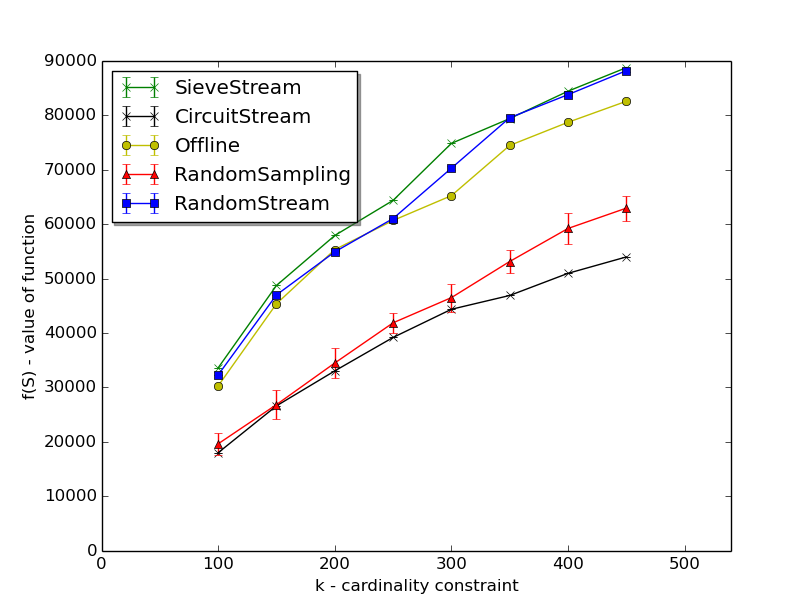
\includegraphics[width=0.5\textwidth]{figures/streaming-shuffle}\label{fig:streaming-shuffle}}
    ~~
    \subfloat[][Edges grouped by vertices]{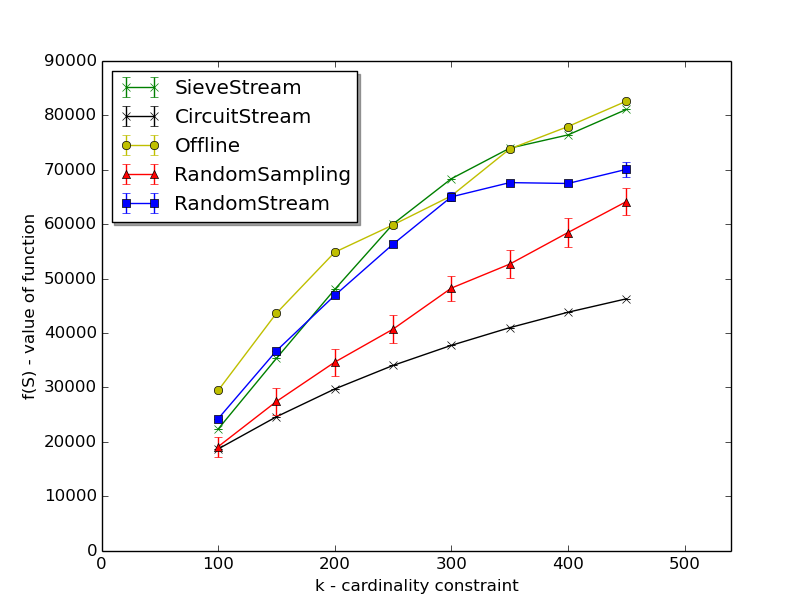
\includegraphics[width=0.5\textwidth]{figures/streaming}\label{fig:streaming-not-shuffle}}    
    \caption{Streaming Algorithms on {\sc Facebook};  $\eps$ is set to be $0.2$ for both \sieveStream and \randomStream; $\gamma$ is set to be $1.0$ for \circuitStream.}
    \label{fig:streaming-facebook}
  \end{figure}
\end{frame}


\subsection{Summary}
\begin{frame}
  \frametitle{Summary of state of the art}
\begin{table}[t]
\centering
\begin{tabular}{|l|l|l|}
\hline
constraint & monotone  &  non-negative \\
\hline
cardinality & $\frac{1-\eps}{2}$ \cite{BMK+14} & $\frac{1 - \eps}{2 + e}$ \cite{CGQ15}, R\\
\hline
matroid & $1/4$ \cite{CK14} & $\frac{1 - \eps}{4 + e}$ \cite{CGQ15},  R \\
\hline
matching & $4/31$ \cite{CK14} & $\frac{1 - \eps}{12 + \eps}$ \cite{CGQ15}, R \\
\hline
intersection of $p$ matroids & $\frac{1}{4p}$ \cite{CK14} & $\frac{(1 - \eps)(p - 1)}{5p^2 -4p + \eps}$ \cite{CGQ15}, R\\
\hline
$p$-matchoid & $\frac{1}{4p}$ \cite{CGQ15} & $\frac{(1-\eps)(2-o(1))}{(8+e)p}$ \cite{CGQ15}, R\\
\hline
\end{tabular}
\caption{Best known approximation bounds for submodular maximization in streaming model. Bounds for randomized algorithms that hold in expectation are marked (R).}
\label{table:streaming}
\end{table}

\end{frame}



% \begin{frame}
% \frametitle{References}
% \footnotesize{
% \begin{thebibliography}{99} % Beamer does not support BibTeX so references must be inserted manually as below
% \bibitem[Smith, 2012]{p1} John Smith (2012)
% \newblock Title of the publication
% \newblock \emph{Journal Name} 12(3), 45 -- 678.
% \end{thebibliography}
% }
% \end{frame}

%------------------------------------------------

%------------------------------------------------
\section{Distributed Submodular Maximization}
%------------------------------------------------
\subsection{The model}
\begin{frame}
  \frametitle{The model}
  \begin{block}{Crash Introduction to MapReduce}
  
  \begin{itemize}
  \item the data is represented as $\langle$key, value$\rangle$ pairs that are distributed across $m$ machines
    \item a computation in this model proceeds in rounds. In each round, there will be two phases.
      \item \emRed{Map phase:} each pair $\langle$key, value$\rangle$ is mapped by a user-defined hash function to $\langle$hash(key), value$\rangle$, all pairs are then shuffled and sent to different machines
      \item \emRed{Reduce phase:} each machine performs computation on the pairs it received as the output or the input of the next round
  \end{itemize}
  \end{block}
  \pause
  \begin{block}{If you do not know MapReduce model ...}
    Think of it as a group of machines with one machine as the coordinator/center node.    
  \end{block}
\end{frame}

\subsection{The framework}

\begin{frame}
  \frametitle{{\sc GreeDi}-based algorithms}
  \begin{block}{framework of {\sc GreeDi}-based algorithms}
    $m$ -  the number of machines; $C \in \bbZ^+$ is an parameter;  $k$ - the cardinality constraint. The algorithm goes as follows:
    \begin{itemize}
    \item Randomly assign each $v$ to $C$ out of $m$ machines, we obtain subsets $V_1, \ldots, V_m$
    \item Let $\alg$ be an offline algorithm, $k'$ be a cardinality constraint. Run $\alg$ on each $V_i$ with constraint $k'$, we obtains $U_1, U_2, \ldots, U_m$ as results.
    \item Let $U = \cup_i S_i$, run $\alg$ on $U$ with parameter $k$, we obtain $S$ as the result. Also run $\alg$ on $U_1, \ldots, U_m$ with parameter $k$ to obtain $S_1, S_2, \ldots, S_m$.
    \item Return the best solution among $S$, $S_1, \ldots, S_m$.
    \end{itemize}

  \end{block}
\end{frame}


\begin{frame}
  \frametitle{Some theories about the {\sc GreeDi}-Based Algorithms}
  \begin{block}{some theories (informal)}
    \begin{itemize}
    \item use the standard greedy algorithm as $\alg$, $k' = k$, $C = 1$, the {\sc GreeDi}-Based algorithm gives $\frac{1-e^{-1}}{2}$-approximation.
    \item increasing $k'$ or $C$ would \textbf{slightly} increase the approximation ratio (in worse case!), but not too much
    \end{itemize}
  \end{block}
  
\end{frame}

\subsection{Experiment}

\begin{frame}
  \frametitle{experiment}
  \begin{figure}[h!]
     \centering
     \subfloat[][Different multiplicity $C$; set $k' = k$; number of machines is $20$.]{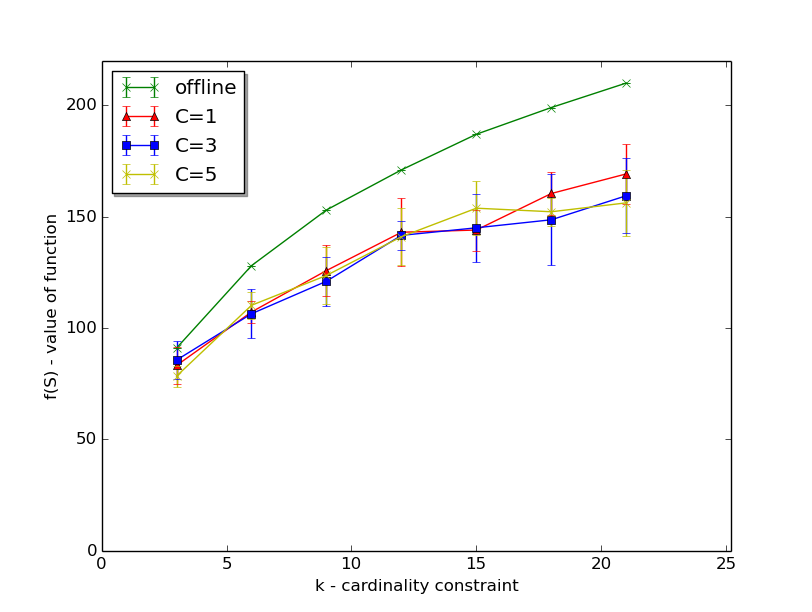
\includegraphics[width=0.5\textwidth]{figures/C-acc}\label{fig:dist-C-acc}}
     ~~
     \subfloat[][Different $k'$; $C$ is set to be $1$; number of machines is set to be $20$.]{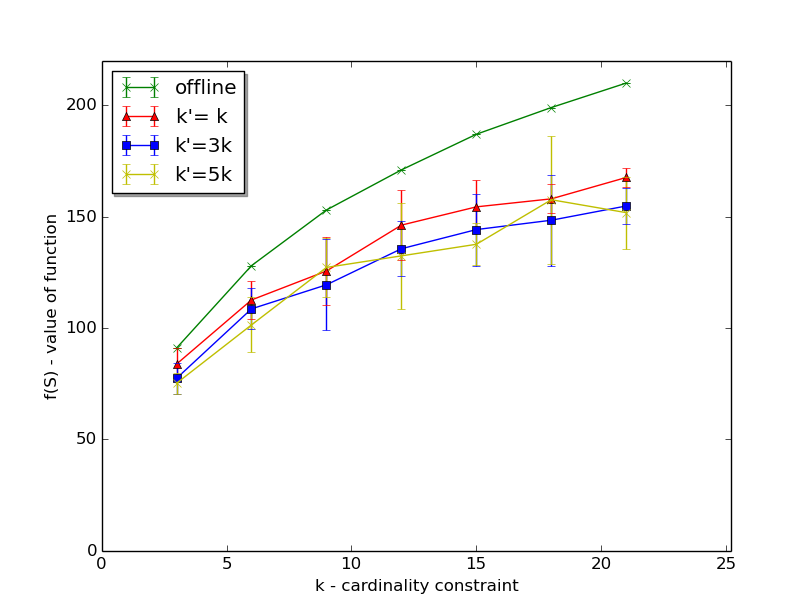
\includegraphics[width=0.5\textwidth]{figures/kk-acc}\label{fig:dist-kk-acc}}    
     \caption{{\sc GreeDi}-based Algorithms on {\sc Accidents} dataset.}
     \label{fig:distributed-accidents}
\end{figure}

\end{frame}



\subsection{Summary}
\begin{frame}
\frametitle{Summary of state of the art}
\begin{table}
\centering
\begin{tabular}{|l|l|l|l|}
\hline
constraint & rounds  &  approx. & reference \\
\hline
\multirow{3}{*}{cardinality} & $O(\frac{\log n}{\eps})$& $1-e^{-1}-\eps$ & \cite{KMV+15}\\
\cline{2-4}
                             & $2$ & $0.545$ & \cite{MZ15} \\
\cline{2-4}
                             & $O(1/\eps)$ & $1 - e^{-1}-\eps$ & \cite{BAN+2015new} \\

\hline


\multirow{3}{*}{matroid}     & $O(\frac{\log n}{\eps})$ & $1/2 - \eps$ & \cite{KMV+15} \\
\cline{2-4}
                             & $2$ & $1/4$ & \cite{DEN+15} \\
\cline{2-4}
                             & $O(1/\eps)$ & $1 - e^{-1}-\eps$ & \cite{BAN+2015new} \\
\hline
\multirow{3}{*}{p-system}     & $O(\frac{\log n}{\eps})$ & $\frac{1}{p+1} - \eps$ & \cite{KMV+15} \\
\cline{2-4}
                            & $2$  & $\frac{1}{2(p + 1)}$ & \cite{DEN+15} \\
\cline{2-4}      
                           & $O(1/\eps)$ & $\frac{1}{p + 1} - \eps$ & \cite{BAN+2015new}\\
\hline
\end{tabular}
\caption{Best known algorithms  for monotone submodular maximization in the MapReduce model. All algorithms are randomized.}
\label{table:distributed}
\end{table}

\end{frame}


\begin{frame}
\Huge{\centerline{Question? Thank you!}}
\end{frame}

%----------------------------------------------------------------------------------------



\bibliographystyle{abbrv}
\bibliography{survey}

\end{document} 